\subsection*{\textbf{RQ4: What are developers' perceptions of why
		delivery delay happens? }}

\begin{sloppypar}
Our findings about developers' perceptions of the causes of delivery delay is
divided into the following themes: {\em (i) development activities}, {\em (ii)
decision making}, {\em (iii) risk}, {\em (iv) frustration}, and {\em (v) team
collaboration}. After discussing each theme below, we present a quantitative
analysis of the factors that can impact delivery delay using the responses to
{\em question~\#13} (see our \hyperref[ch5:datacollection2]{data collection}
process).\\ 

\noindent\textit{\textbf{Theme~1---Development activities.}}\theme{th:1} 
The number of tests that should be executed was a recurrent theme among
participants. For instance, several participants stated that {\em additional
testing}$^{(12)}$ should be executed in order to avoid delivery delay. {\em
P17} states that the lack of {\em ``actual user testing beyond what QA can
provide''} can lead to delivery delay. Additionally, according to {\em F15},
{\em ``the most common reason is that testing was incomplete''} and according to {\em
P19}, delivery delay may happen because {\em ``testing has been too
narrow''.} Finally, {\em E32} voices concerns about integration testing: {\em
``No integration tests has been done.''} Such observations bring us back to a
core software engineering problem of when is testing
sufficient?~\cite{beller2015much,alghamdi2016automated}.

Other recurrent themes that emerged during our qualitative analysis are {\em
workload}$^{(7)}$ and {\em code review}.$^{(7)}$ For example, {\em E30} states
that {\em ``As the delayed completed issues stack up, they are harder to
integrate (the codebase is constantly changing, merge issues might emerge).''}
Interestingly, our statistical models in our prior work (see
\hyperref[ch:study12]{Chapter}~\ref{ch:study12})
indicate {\em workload}$^{(7)}$ as a metric that shares a strong relationship
with delivery delay. As for {\em code review},$^{(7)}$ the {\em
``Unavailability of the lead/reviewer/[Project Management Committee] (PMC)''} is
a reason of delivery delay that is pointed out by {\em E26}, while {\em F08}
argues that a {\em ``prompt code reviews [may] help''} to avoid delivery
delays~\cite{mcintosh2016emse}.\\

\noindent\textit{\textbf{Theme~2---Decision making.}}\theme{th:2} Decision making refers to the
activities that are not directly related to software construction, but can
influence the speed at which software is shipped. For example, how early a
codebase should be ``frozen''? Which issues should be prioritized? The {\em
timing}$^{(9)}$ and {\em prioritization}$^{(9)}$ are the recurrent themes in
our survey responses. For instance, two of the participants stated that issues
can be delayed because they are addressed {\em ``too late in the release
cycle''} ({\em E28}) or because they were addressed in a {\em ``long release
cycle.''} Also, {\em F12}'s opinion about how to avoid delivery delay is to
{\em ``test [addressed issues] early using real users (\eg on the pre-release
channels).''} Regarding {\em prioritization},$^{(9)}$ {\em E28} argues that team
members should {\em ``try to complete most important things early in the release
cycle''} to avoid delivery delay. Additionally, {\em F07} points out how
re-prioritization of issues is important: {\em ``[...] prioritizing and
re-prioritizing tasks to be sure you are building things on time [...].''}\\

\noindent\textit{\textbf{Theme~3---Risk.}}\theme{th:3} The risk that is associated with shipping
addressed issues may generate delivery delay according to our participants.
Among the risky addressed issues, the ones that have {\em
compatibility}$^{(12)}$ concerns are the most recurrent in this theme. For example, when
asked about reasons that may lead to delivery delay, {\em F12} calls
attention to issues that {\em ``break third-party websites''} and that can
generate {\em ``incompatibility with third-party software that users install.''}
Another risk that is associated with delivery delay is {\em stability}.$^{(9)}$
For instance, {\em F03} states that {\em ``when there are regressions
noticed during Aurora/Beta cycles,''} an addressed issue will likely skip the
upcoming official release.\\

\noindent\textit{\textbf{Theme~4---Frustration.}}\theme{th:4} Delivery delay may generate
frustration to both users and developers of the software. The majority of users'
frustration comes from their {\em expectation}$^{(20)}$ about the addressed
issues. {\em F07} makes an interesting analogy to explain user frustration: {\em
``as a user, it's like when you are waiting your suitcase in the airport to
come out on the belt. You know it has to be there, but you keep waiting.''}
{\em F14} also provides another analogy: {\em ``it's like a gift for Christmas,
but the day of Christmas is postponed.''} On the other hand, developers may get
frustrated for other reasons than users. The greatest frustration source for
developers is the feeling of {\em useless/unreleased work}.$^{(9)}$ According to
{\em F09}, when an addressed issue is delayed, a developer {\em ``feels like
[their] work is meaningless.''} {\em F04} complements {\em F09} by stating that
{\em ``it is frustrating to work on something and not see it shipped.''} \\

\noindent\textit{\textbf{Theme~5---Collaboration with other teams.}}\theme{th:5}
Delivery delay may also occur due to
the overhead that is introduced when {\em collaboration}$^{(10)}$ is needed
between teams. For example, when asked to recall a delayed addressed
issue, {\em F23} answers that {\em ``sometimes, issues that require cross-team
cooperation may be delayed when the issue is differently prioritized by each
team.''} The {\em marketing}$^{(5)}$ team is mentioned recurrently when
delivery delay occurs due to other teams' collaboration. For instance,
according to {\em F21}, delivery delay {\em ``generally happens when
marketing wants to make a splash.''} {\em F08} also corroborates  {\em F21} by
stating that {\em ``product management [may] change their mind about the
desirability of a feature, or would like to time the release of the feature with
certain external events for marketing reasons.''}\\

\noindent\textit{\textbf{Observation~7---The time at which an issue is addressed
during a release cycle and the issue severity are the factors that receive the
highest ratings of importance.}}\observation{obs:7} In {\em
question~\#13} of our survey, we ask participants to rate the degree to which a
factor is related to delivery delay. The factors that we list are: the
reporter, the resolver, the priority, the severity, the number of comments, the
number of modified files, the number of modified LOC, and the time at which an
issue was addressed during a release cycle. The responses to {\em question~\#13}
are based on a 5-points-Likert scale, \ie participants rate factors using ranks from 1
(strongly disagree) to 5 (strongly agree). 

\begin{figure}
	\centering
	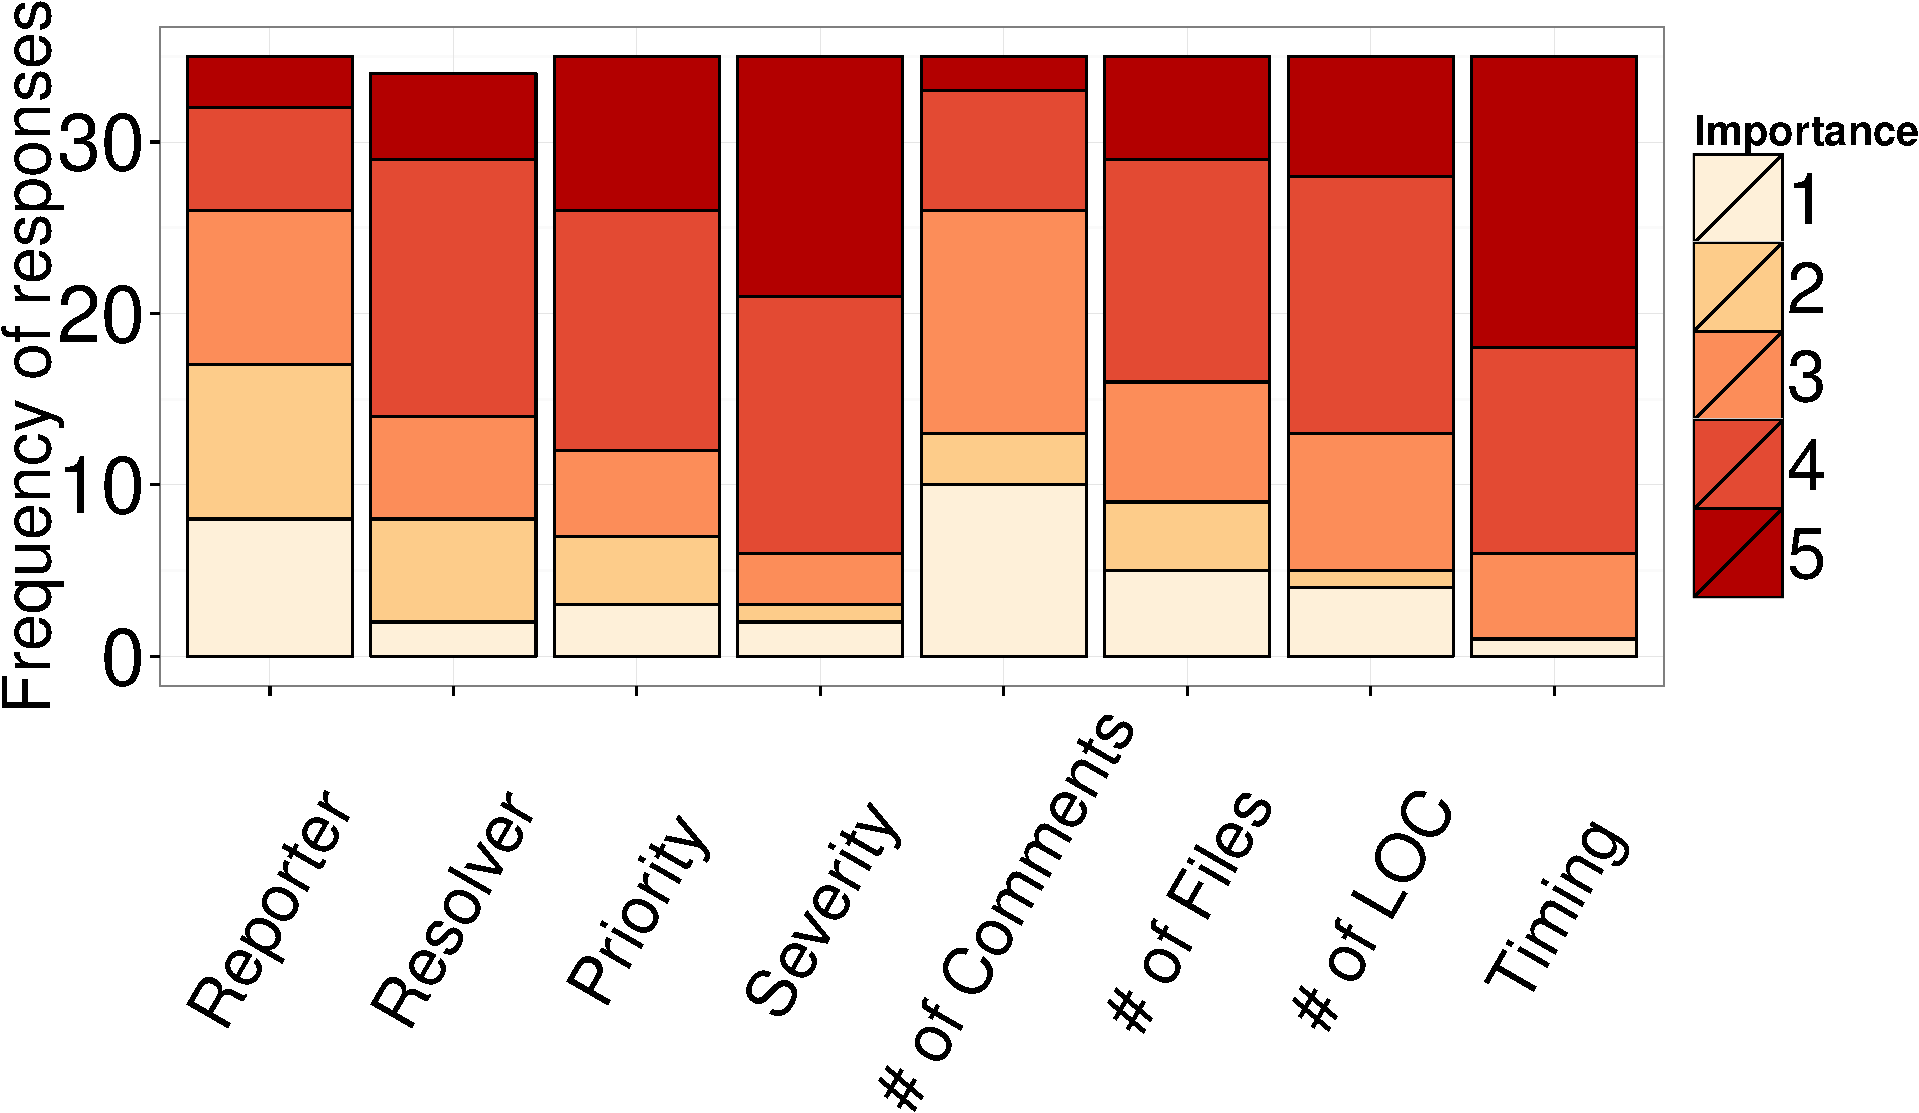
\includegraphics[width=0.80\textwidth,keepaspectratio]
	{chapters/chapter5/figures/rank_frequency.pdf}
	\caption{Frequency of ranks per factor.}
	\label{fig:rank_frequency}
\end{figure}

\begin{table}
	\footnotesize
	\centering
	\caption{Rating of factors related to delivery delay. The highest
		ratings are in bold.
		\label{tbl:factors}
	}
	\begin{tabular}{lr}
		\hline 
		\textbf{Factor} & \textbf{Average rating (mean)}\tabularnewline
		\hline 
		\hline 
		Time at which an issue is addressed during a release cycle (timing) & \textbf{4.257}\tabularnewline
		\hline 
		Severity & \textbf{4.086}\tabularnewline
		\hline 
		Priority & 3.629\tabularnewline
		\hline 
		Number of LOC & 3.571\tabularnewline
		\hline 
		Resolver & 3.441\tabularnewline
		\hline 
		Number of files & 3.314\tabularnewline
		\hline 
		Number of comments & 2.657\tabularnewline
		\hline 
		Reporter & 2.629\tabularnewline
		\hline 
	\end{tabular}
\end{table}

In \hyperref[fig:rank_frequency]{Figure}~\ref{fig:rank_frequency}, we show the
frequency of each rank per factor, while  we show the average rating of each
factor in \hyperref[tbl:factors]{Table}~\ref{tbl:factors}. We observe that the
factors that receive the highest ranks are {\em severity} and {\em timing}. This
result is in agreement with our regression models that are presented in RQ3, in
which {\em cycle queue rank} is one of the most influential variables
(see \hyperref[obs:6]{Observation}~\ref{obs:6}). Indeed, during the interview, {\em
P06} further explains that if an issue that is risky is addressed in the end of
a release cycle, such an issue is likely to be delayed to the next cycle, so
that it can receive additional testing.

\begin{figure}
	\centering
	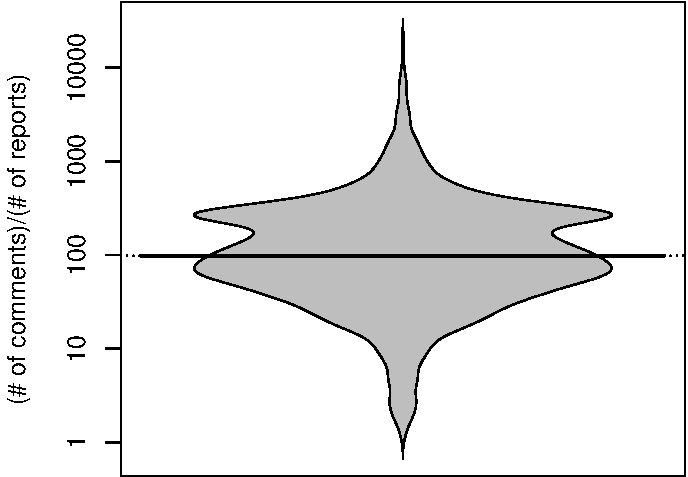
\includegraphics[width=.8\textwidth,keepaspectratio]
	{chapters/chapter5/figures/comments_ratio.pdf}
	\caption{Distribution of number of comments normalized by the number of
	reported issues.}
	\label{fig:comments_ratio}
\end{figure}

On the other hand, the factors with the lowest ranks are {\em reporter}, and
{\em \# of comments}. We also asked our interviewees about these lower ratings.
One of our interviewees explained that the reporter of an issue might influence
delivery delay only in cases in which the reporter is also a Firefox
employee. In these cases, the reporter will address the issue her/himself, which
can speed up the shipping process.\footnote{We did not observe a statistically
	significant difference in delivery delays between issues that are
addressed by the reporters themselves and issues that are addressed by a
different team member.} As for the {\em \# of comments}, another interviewee
clarified that there are several passionate people on bugs that can inflate the
number of comments even if the issue is easy to ship. For each reporter, we
normalize the number of his/her comments by the number of his/her reported issues.  We
plot the distribution of the normalized number of comments in
\hyperref[fig:comments_ratio]{Figure}~\ref{fig:comments_ratio}. The median
number of comments per reported issue is 98. Indeed, we observe reporters with a
great number of comments (\eg 500 to 10,000 comments) per reported issue.
This result suggest that the perception of our interviewee is likely to be true.

\begin{table}
	\scriptsize
	\centering
	\caption{$P$-$values$ of the comparisons between factors. Values in bold are $<$ 0.05.
		\label{tbl:pvalues_factors}
	}
	\begin{tabular}{lrrrr}
		\hline 
		Factor x Factor & Reporter & Resolver & Priority & Severity\tabularnewline
		\hline 
		\hline 
		Reporter & --- & 1.2$e^{-1}$ & \textbf{1.3$e^{-2}$} & \textbf{1.4$e^{-5}$} \tabularnewline
		\hline 
		Resolver & 1.2$e^{-1}$ & --- & 1 & 1.2$e^{-1}$ \tabularnewline
		\hline 
		Priority & \textbf{1.3$e^{-2}$} & \textbf{1.3$e^{-2}$} & --- & 4.8$e^{-1}$ \tabularnewline
		\hline 
		Severity & \textbf{1.4$e^{-5}$} & 1.2$e^{-1}$ & 4.7$e^{-1}$ & ---\tabularnewline
		\hline 
		\# of Comments & 4.8$e^{-1}$ & 1.2$e^{-1}$ & \textbf{1.4$e^{-2}$} & \textbf{1.6$e^{-5}$} \tabularnewline
		\hline 
		\# of Files & 1.8$e^{-1}$ & 7.9$e^{-1}$ & 1 & 6.6$e^{-2}$ \tabularnewline
		\hline 
		\# of LOC & \textbf{3.0$e^{-2}$} & 1 & 1 & 2.8$e^{-1}$ \tabularnewline
		\hline 
		Timing & \textbf{8.0$e^{-7}$} & \textbf{3.2$e^{-2}$} & 1.8$e^{-1}$ & 1\tabularnewline
		\hline 
		\hline
		Factor x Factor & \# of Comments & \# of Files & \# of LOC & Timing\tabularnewline
		\hline 
		Reporter & 4.8$e^{-1}$ & 1.8$e^{-1}$ & \textbf{3.0$e^{-2}$} & \textbf{8.1$e^{-7}$} \tabularnewline
		\hline 
		Resolver & 1.2$e^{-1}$ & 7.9$e^{-1}$ & 1 & \textbf{3.2$e^{-2}$} \tabularnewline
		\hline 
		Priority & \textbf{1.4$e^{-2}$} & 1 & 1 & 1.8$e^{-1}$ \tabularnewline
		\hline 
		Severity & \textbf{1.6$e^{-5}$} & 6.6$e^{-2}$ & 2.8$e^{-1}$ & 1\tabularnewline
		\hline 
		\# of Comments & --- & 1.7$e^{-1}$ & \textbf{3.3$e^{-2}$} & \textbf{9.6$e^{-7}$} \tabularnewline
		\hline 
		\# of Files & 1.7$e^{-1}$ & --- & 1 & \textbf{1.4$e^{-2}$} \tabularnewline
		\hline 
		\# of LOC & 3.3$e^{-2}$ & 1 & --- & 1.1$e^{-1}$ \tabularnewline
		\hline 
		Timing & \textbf{9.6$e^{-7}$} & \textbf{1.4$e^{-2}$} & 1.1$e^{-1}$ & ---\tabularnewline
		\hline 
	\end{tabular}
\end{table}

A Kruskal Wallis test indicates that the difference in ratings between metrics
are statistically significant ($p=0.01507$).
\hyperref[tbl:pvalues_factors]{Table}~\ref{tbl:pvalues_factors} shows the
Bonferroni corrected $p$-$values$ of the Dunn tests. We observe that the {\em
timing} factor has significant larger response values than all the other factors except
the {\em severity}, {\em priority}, and {\em LOC} factors ($p<0.05$).

We also use Spearman's $\rho$ to correlate the rating of the factors with (i)
general experience ({\em question \#1}) and (ii) project experience ({\em
question \#2}). The only statistically significant correlation that we observe is
between the {\em timing} factor and general experience. We achieve a negative
correlation of -0.36 ($p=0.03235$). This result suggests that less
experienced participants tend to report that the time at which an issue is
addressed during a release cycle plays a more important role in delivery
delay. One of our interviewees explains this observation by stating that {\em
``when an issue is addressed early in the release cycle, it should have more
time to be tested before integration,''} which can be helpful for fixes
from less experienced resolvers. Finally, we also correlate the responses
to {\em question~\#6} with general and project experience. However, no
significant correlations were found.\\
\end{sloppypar}

\conclusionbox{Our survey participants report that the delivery of addressed
issues may be delayed due to reasons that are related to the development
activities, decision making, team collaboration, or risk. Moreover, delivery
delay likely lead to user/developer frustration.}

